\chapter{Astrophysics}\label{ch:b3:astrophysics}

% Provenance (not for print): the astrophysics option offered across the
% surveyed third-year curricula, built here as a capstone that reuses the
% whole volume (Fermi gas -> white dwarfs, nuclear -> stellar burning,
% Planck law -> CMB, Saha -> recombination).

Every chapter of this book has been rehearsing for this one. Stars
are self-gravitating gas balls run by the hydrostatics of the Year 1
volume, fired by \cref{ch:b3:nuclear-physics}'s tunnelling, shining
by \cref{ch:b3:photons-phonons}'s Planck law; dead stars are
\cref{ch:b3:quantum-statistics}'s degenerate Fermi gases the size of
cities; and the universe itself is a cooling thermal system whose
baby picture --- the microwave background --- is the most perfect
blackbody ever measured. This closing chapter assembles the whole
volume into the biggest possible laboratory: how stars live, how
they die, what they leave behind, and how the expanding universe
that contains them began as physics we have already done.

\section{A star is a balance}

\begin{proposition}[Hydrostatic equilibrium]\label{prop:b3:astrophysics:hydrostatic}
\index{hydrostatic equilibrium (stellar)}\index{stellar structure}
A star neither collapses nor disperses: at every radius, the
pressure gradient carries the weight of the gas above. For the
mass $m(r)$ inside radius $r$,
\[
\frac{\dd P}{\dd r} = -\frac{Gm(r)\rho(r)}{r^2} .
\]
Estimated across the whole Sun, $P_{\text{c}} \sim GM^2/R^4 \sim
\qty{e15}{Pa}$ and, via the ideal-gas law, $T_{\text{c}} \sim
10^7\,\unit{K}$ (\cref{exo:b3:astrophysics:1}) --- precisely the
temperature at which \cref{exo:b3:nuclear-physics:11}'s protons
begin to tunnel. That is no coincidence but a thermostat: a star
\emph{must} contract and heat until its core ignites, and fusion
then holds the balance for millions to billions of years. Stars
have negative heat capacity --- lose energy, contract, get
\emph{hotter} (\cref{exo:b3:astrophysics:5}) --- which is why
gravity always wins in the end.
\end{proposition}

\begin{proof}
A shell $[r, r + \dd r]$ of area $A$ feels pressure $P(r)A$ from
below, $P(r + \dd r)A$ from above, and weight $g\rho A\,\dd r$
with $g = Gm(r)/r^2$ (only the interior mass pulls, by Gauss's
theorem for gravity). Equilibrium of the three gives the stated
equation.
\end{proof}

\begin{omfigure}
\begin{tikzpicture}[scale=1.0]
  \fill[omExo!14] (0,0) circle (2.2);
  \fill[omExo!30] (0,0) circle (1.15);
  \draw[omDef, thick] (0,0) circle (2.2);
  \draw[omDef!60] (0,0) circle (1.15);
  \node[font=\scriptsize, align=center] at (0,0)
    {core\\$10^7\,\unit{K}$: fusion};
  % pressure arrows outward
  \foreach \ang in {25,115,205,295}
    \draw[->, omThm, thick] (\ang:1.25) -- (\ang:1.8);
  \node[omThm, font=\scriptsize, anchor=west] at (2.5,0.85)
    {pressure pushes out};
  % gravity arrows inward
  \foreach \ang in {70,160,250,340}
    \draw[->, omDef, thick] (\ang:2.75) -- (\ang:2.3);
  \node[omDef, font=\scriptsize, anchor=west] at (2.5,-0.85)
    {gravity pulls in};
\end{tikzpicture}

{\small A star, drawn as its own free-body diagram. Fusion powers
the pressure that carries the star's own weight; the two forces
negotiate for ten billion years --- and every stellar fate in this
chapter is what happens when one of them runs out of arguments.}
\end{omfigure}

\section{The lives of stars}

\begin{definition}[The Hertzsprung--Russell diagram]\label{def:b3:astrophysics:hr}
\index{Hertzsprung--Russell diagram}\index{main sequence}
Plot stars by surface temperature (hot on the \emph{left}, by
convention) against luminosity, both from
\cref{ch:b3:photons-phonons}'s blackbody laws, and they refuse to
scatter: ninety percent crowd onto the \emph{main sequence}, the
diagonal band of hydrogen-burners, ordered purely by mass ---
heavier means hotter \emph{and} disproportionately brighter
($L \propto M^{3.5}$), hence shorter-lived
($t \propto M/L \propto M^{-2.5}$:
\cref{exo:b3:astrophysics:4}). Off the band live the
plot's exceptions and endings: cool but enormous \emph{giants}
(top right), and hot but tiny \emph{\omterm{ex:b3:quantum-statistics:dwarf}{white dwarfs}} (bottom left)
--- because at fixed temperature, by $L = 4\pi R^2\sigma T^4$,
luminosity is a measure of \emph{size}. The HR diagram is not a
map of kinds but of \emph{ages}: a star's dot drifts across it as
its fuel runs down.
\end{definition}

\begin{omfigure}
\begin{tikzpicture}
  \begin{axis}[omaxis, axis x line=bottom, axis y line=left,
    width=9.8cm, height=6.8cm, xmin=0, xmax=10, ymin=-4.6, ymax=6.4,
    xlabel={surface temperature (hot $\to$ cool)},
    ylabel={$\log_{10}(L/L_\odot)$},
    xlabel style={at={(axis description cs:0.5,-0.08)}, anchor=north},
    xtick=\empty, ytick={-4,-2,0,2,4,6}, clip=false]
    % main sequence band
    \addplot[omDef, line width=5pt, opacity=0.28, domain=0.6:9.4]
      {5.0 - 1.05*x};
    \addplot[omDef, thick, domain=0.6:9.4] {5.0 - 1.05*x};
    % sun
    \fill[omExo] (axis cs:4.76,0) circle (2pt);
    \node[omExo, font=\scriptsize, anchor=north east] at (axis cs:4.6,-0.4)
      {Sun};
    % giants
    \fill[omThm!25] (axis cs:8.1,3.4) ellipse (1.35 and 1.0);
    \node[omThm, font=\scriptsize] at (axis cs:8.1,3.4) {giants};
    % white dwarfs
    \fill[gray!25] (axis cs:2.6,-3.2) ellipse (1.5 and 0.75);
    \node[font=\scriptsize] at (axis cs:2.6,-3.2) {white dwarfs};
    \node[omDef, font=\scriptsize, rotate=-38, anchor=south] at
      (axis cs:2.6,2.5) {main sequence};
  \end{axis}
\end{tikzpicture}

{\small The \omterm{def:b3:astrophysics:hr}{Hertzsprung--Russell diagram}. The \omterm{def:b3:astrophysics:hr}{main sequence} is the
hydrogen-burning band, a mass ladder read top-left (blue,
profligate, dead in megayears) to bottom-right (red, frugal,
outliving the universe so far). Giants and \omterm{ex:b3:quantum-statistics:dwarf}{white dwarfs} are not
oddities but chapters: the same star visits all three regions.}
\end{omfigure}

\begin{remark}[How stars age, and what they leave]\label{rem:b3:astrophysics:evolution}
\index{red giant}\index{supernova}\index{nucleosynthesis (stellar)}
When the core's hydrogen is spent, the thermostat logic replays:
the core contracts and heats, helium ignites (fusing to carbon
and oxygen), the envelope bloats a hundredfold --- a \omterm{rem:b3:astrophysics:evolution}{red giant}.
A Sun-like star stops there: it sheds its envelope and retires
as a \omterm{ex:b3:quantum-statistics:dwarf}{white dwarf}. A star above $\approx8M_\odot$ keeps igniting
new fuels in onion shells until the core is \emph{iron} ---
\cref{prop:b3:nuclear-physics:binding}'s summit, from which no
fusion returns energy. The dead core collapses in a second; the
rebound and the neutrino flood blow the star apart: a
\emph{supernova}, briefly outshining its galaxy, forging the
elements beyond iron by neutron capture and broadcasting the lot
into the clouds that build the next generation of stars and
planets. The calcium in your bones and the iron in your blood
took this route (\cref{pb:b3:astrophysics:1}): chemistry is
recycled astrophysics.
\end{remark}

\section{The corpses: matter at its limits}

\begin{proposition}[White dwarfs and neutron stars]\label{prop:b3:astrophysics:compact}
\index{white dwarf}\index{neutron star}\index{Chandrasekhar mass}\index{black hole}\index{Schwarzschild radius}
What holds a star that no longer burns? Quantum mechanics. A
\emph{\omterm{ex:b3:quantum-statistics:dwarf}{white dwarf}} is a solar mass of carbon and oxygen propped
up by its \emph{electron \omterm{thm:b3:quantum-statistics:fermi}{degeneracy pressure}} --- the $T = 0$
Fermi pressure of \cref{ch:b3:quantum-statistics} --- at the size
of the Earth and a tonne per teaspoon. Pauli's support has a
ceiling: above the \emph{\omterm{prop:b3:astrophysics:compact}{Chandrasekhar mass}} $M_{\text{Ch}}
\approx 1.4\,M_\odot$, the electrons go relativistic and the
pressure loses the race (a result we state, not derive). Beyond
it, electrons are crushed into protons and a \emph{\omterm{prop:b3:astrophysics:compact}{neutron star}}
forms: neutron degeneracy plus nuclear repulsion holding
$\sim1.4\,M_\odot$ in a dozen kilometres at
\cref{def:b3:nuclear-physics:nuclide}'s nuclear density --- a
city-sized nucleus, spinning up to milliseconds and beaming like
a lighthouse (a \emph{pulsar}). And beyond about $3\,M_\odot$
nothing known resists: the star falls inside the radius at which
escape needs light speed,
\[
R_{\text{s}} = \frac{2GM}{c^2}
\qquad (\qty{3}{km}\text{ per solar mass}) ,
\]
a \emph{\omterm{prop:b3:astrophysics:compact}{black hole}} --- gravity's final word, and general
relativity's doorstep, one volume beyond this one.
\end{proposition}
\admitted

\begin{omfigure}
\begin{tikzpicture}[scale=1.0]
  % log-scale size ladder
  \draw[omDef, fill=omExo!18, thick] (0,0) circle (1.9);
  \node[font=\scriptsize, align=center] at (0,-2.35)
    {Sun\\$7\times10^5$ km};
  \draw[omDef, fill=omDef!15, thick] (4.4,0) circle (0.55);
  \node[font=\scriptsize, align=center] at (4.4,-2.35)
    {white dwarf\\$\sim\qty{7000}{km}$};
  \draw[omThm, fill=omThm!18, thick] (7.3,0) circle (0.16);
  \node[font=\scriptsize, align=center] at (7.3,-2.35)
    {neutron star\\$\sim\qty{12}{km}$};
  \fill (9.7,0) circle (0.06);
  \node[font=\scriptsize, align=center] at (9.7,-2.35)
    {black hole\\$R_{\text{s}} \sim \qty{4}{km}$};
  \node[font=\scriptsize, gray, anchor=south, align=center] at (4.85,1.55)
    {similar mass, ever fiercer gravity\\(sizes not to scale)};
\end{tikzpicture}

{\small One solar mass, four sizes. Thermal pressure holds the
Sun; electron degeneracy the \omterm{ex:b3:quantum-statistics:dwarf}{white dwarf}; neutron degeneracy the
\omterm{prop:b3:astrophysics:compact}{neutron star}; nothing holds the \omterm{prop:b3:astrophysics:compact}{black hole}. Each step multiplies
surface gravity by ten thousand or so --- and the physics needed
to stand on it.}
\end{omfigure}

\section{The expanding universe}

\begin{definition}[Hubble's law and the hot beginning]\label{def:b3:astrophysics:hubble}
\index{Hubble's law}\index{cosmic microwave background}\index{Big Bang nucleosynthesis}
Every distant galaxy recedes, at speed proportional to distance:
\[
v = H_0d , \qquad H_0 \approx \qty{70}{km/s}
\text{ per megaparsec} .
\]
This is not an explosion \emph{into} space but an expansion
\emph{of} space --- run it backwards and everything was once
dense and hot: $1/H_0 \approx 14$ billion years ago
(\cref{exo:b3:astrophysics:9}). The early universe is this book
replayed at speed. At one second it is a \unit{MeV} particle soup
(\cref{ch:b3:particle-physics}); in the first minutes,
\cref{ch:b3:nuclear-physics} runs wild and freezes out
\emph{one quarter helium by mass} --- predicted by a Boltzmann
factor, observed everywhere
(\cref{exo:b3:astrophysics:11}). At 380\,000 years and
\qty{3000}{K}, Saha's equation
(\cref{prop:b3:grand-canonical:saha}) lets electrons finally settle
onto protons; the fog clears, and that last-scattered light ---
stretched a thousandfold by expansion --- arrives today as the
\emph{cosmic microwave background}: a \qty{2.725}{K} Planck
spectrum (\cref{ch:b3:photons-phonons}), the oldest photograph
there is. What the picture also shows: galaxies spin and cluster
as if steered by \emph{\omterm{rem:b3:particle-physics:higgs}{dark matter}} no detector has caught, and
the expansion \emph{accelerates} under a \emph{dark energy}
nobody has explained --- the ninety-five percent of the budget
this book cannot yet write.
\end{definition}

\begin{omfigure}
\begin{tikzpicture}
  \begin{axis}[omaxis, axis x line=bottom, axis y line=left,
    width=9.6cm, height=5.8cm, xmin=0, xmax=105, ymin=0, ymax=8.4,
    xlabel={distance (\unit{Mpc})},
    ylabel={recession speed ($10^3\,\unit{km/s}$)},
    xlabel style={at={(axis description cs:0.5,-0.1)}, anchor=north},
    xtick={25,50,75,100}, ytick={2,4,6,8}, clip=true]
    \addplot[omDef, thick, domain=0:103] {0.07*x};
    \addplot[only marks, mark=*, mark size=1.4pt, omThm]
      coordinates {(9,0.75) (17,1.05) (24,1.85) (31,2.0) (39,2.9)
        (46,3.05) (54,3.95) (61,4.1) (69,5.05) (76,5.15)
        (84,6.05) (91,6.2) (98,7.0)};
    \node[omDef, font=\scriptsize, anchor=north west] at (axis cs:57,3.6)
      {slope $H_0$};
  \end{axis}
\end{tikzpicture}

{\small \omterm{def:b3:astrophysics:hubble}{Hubble's law}: recession speed against distance, each dot
a galaxy (speeds from Doppler shifts,
\cref{ch:b3:relativistic-kinematics}; distances from standard
candles). The slope is $H_0$; its inverse is, roughly, the age
of the universe.}
\end{omfigure}

\begin{omfigure}
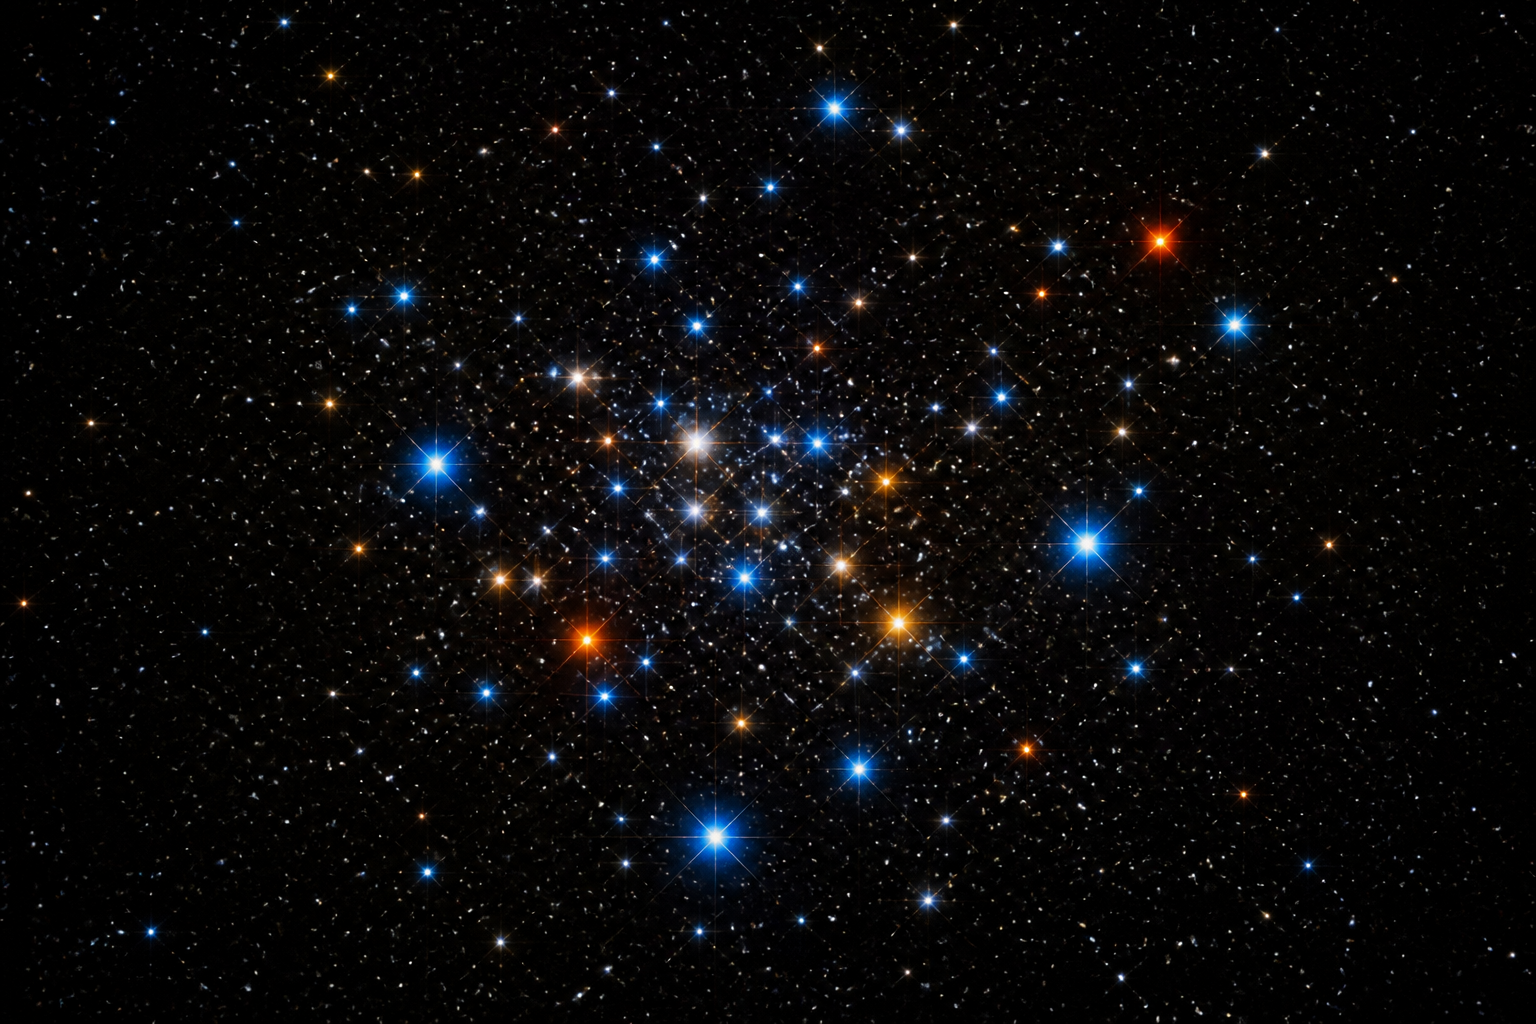
\includegraphics[width=0.58\linewidth]{images/book5/ai/b5-23-star-colors.png}

{\small An open cluster: blue-white profligates and frugal orange dwarfs, born together, ageing at wildly different rates --- the \omterm{def:b3:astrophysics:hr}{Hertzsprung--Russell diagram}, photographed.}
\end{omfigure}

\section{Exercises}

\begin{exercise}[$\star$]\label{exo:b3:astrophysics:1}
The Sun, estimated. $M = \qty{2e30}{kg}$, $R = \qty{7e8}{m}$.
(a) Estimate $P_{\text{c}} \sim GM^2/R^4$. (b) With the mean
density and the ideal-gas law ($P = \rho k_{\text{B}}T/
m_{\text{p}}$), estimate $T_{\text{c}}$. (c) Compare with the
$10^7\,\unit{K}$ ignition threshold of
\cref{exo:b3:nuclear-physics:11}. (d) Why is this agreement a
thermostat rather than a coincidence?
\end{exercise}

\begin{exercise}[$\star$]\label{exo:b3:astrophysics:2}
Weighing light. (a) From the solar constant
\qty{1360}{W/m^2} at $d = \qty{1.5e11}{m}$, compute
$L_\odot$. (b) From $L = 4\pi R^2\sigma T^4$, compute the
surface temperature. (c) Check Wien's peak against the Sun's
visible yellow-green. (d) Which chapter's law did each step use?
\end{exercise}

\begin{exercise}[$\star$]\label{exo:b3:astrophysics:3}
Reading the diagram. Sirius B: $T \approx \qty{25000}{K}$, $L
\approx 0.026\,L_\odot$; Betelgeuse: $T \approx \qty{3500}{K}$,
$L \approx 10^5\,L_\odot$. (a) Place both on the HR diagram. (b)
From $L = 4\pi R^2\sigma T^4$, compute each radius in solar
units. (c) Betelgeuse in the Solar System: which planets are
inside it? (d) What must be holding Sirius B up?
\end{exercise}

\begin{exercise}[$\star$]\label{exo:b3:astrophysics:4}
Live fast, die young. With $L \propto M^{3.5}$ and lifetime
$t \propto M/L$, and the Sun's ten billion years: (a) lifetime
of a $10\,M_\odot$ star; (b) of a $0.5\,M_\odot$ red dwarf ---
compare with the universe's age; (c) why do heavier stars, with
\emph{more} fuel, die \emph{sooner}? (d) What does the shortness
of massive lives imply about where (in a galaxy) supernovae
occur?
\end{exercise}

\begin{exercise}[$\star\star$]\label{exo:b3:astrophysics:5}
Gravity's strange thermodynamics. For a self-gravitating gas
ball the virial theorem (\cref{ch:b3:lagrangian-mechanics})
gives total energy $E = -K$ (minus the kinetic/thermal energy).
(a) Deduce: radiating energy away makes the star \emph{hotter}
--- a negative heat capacity. (b) Estimate the gravitational
energy $GM^2/R$ of the Sun. (c) At today's $L_\odot$, how long
could contraction alone have powered it (the Kelvin--Helmholtz
time)? (d) Geology dates Earth at 4.5 billion years: state the
nineteenth-century paradox and its nuclear resolution.
\end{exercise}

\begin{exercise}[$\star\star$]\label{exo:b3:astrophysics:6}
Anatomy of a \omterm{ex:b3:quantum-statistics:dwarf}{white dwarf}. Take $M = 1\,M_\odot$ at
$R = R_{\text{Earth}} = \qty{6.4e6}{m}$. (a) Compute the mean
density, and a teaspoon's (\qty{5}{mL}) mass. (b) Compute the
surface gravity. (c) \Cref{ch:b3:quantum-statistics}'s
\omterm{thm:b3:quantum-statistics:fermi}{degeneracy pressure} scales as $n^{5/3}$, gravity's need as
$M^2/R^4 \propto n^{4/3}M^{2/3}$: show this implies the
bizarre $R \propto M^{-1/3}$ --- heavier dwarfs are
\emph{smaller}. (d) Explain physically why piling on mass
shrinks the star, and what that portends at the \omterm{prop:b3:astrophysics:compact}{Chandrasekhar
mass}.
\end{exercise}

\begin{exercise}[$\star\star$]\label{exo:b3:astrophysics:7}
Anatomy of a \omterm{prop:b3:astrophysics:compact}{neutron star}. (a) At nuclear density
$\qty{2.3e17}{kg/m^3}$, compute the radius holding
$1.4\,M_\odot$. (b) The pre-collapse core spun once per 25 days
at $R \sim 10^5\,\unit{km}$: use angular-momentum conservation
to estimate the final spin period. (c) Compute the surface
gravity. (d) Flux freezing amplifies the magnetic field as
$B \propto 1/R^2$ (\cref{ch:b3:electromagnetism-in-matter}):
from a stellar \qty{e-2}{T}, what surface field results, and
why do pulsars beam?
\end{exercise}

\begin{exercise}[$\star\star$]\label{exo:b3:astrophysics:8}
The point of no return. (a) Derive $R_{\text{s}} = 2GM/c^2$ from
the Newtonian escape-speed condition $v_{\text{esc}} = c$ (the
honest derivation needs general relativity; the answer,
famously, agrees). (b) Evaluate for the Sun and for the Earth.
(c) The Galaxy's central \omterm{prop:b3:astrophysics:compact}{black hole}: $M = 4\times10^6\,M_\odot$
--- compute $R_{\text{s}}$ and compare with the Sun--Mercury
distance ($\qty{5.8e10}{m}$). (d) Show the mean density inside
$R_{\text{s}}$ falls as $1/M^2$ --- a big enough \omterm{prop:b3:astrophysics:compact}{black hole} is
less dense than water: what does that say about ``crushing''
intuitions?
\end{exercise}

\begin{exercise}[$\star\star\star$]\label{exo:b3:astrophysics:9}
Hubble arithmetic. $H_0 = \qty{70}{km/s}$ per Mpc; $1\,
\text{Mpc} = \qty{3.09e22}{m}$. (a) Convert $H_0$ to SI. (b)
Compute $1/H_0$ in years. (c) A galaxy at \qty{200}{Mpc}: its
recession speed, and the factor by which its light's wavelength
has stretched (small-$z$ Doppler,
\cref{ch:b3:relativistic-kinematics}). (d) Why is $1/H_0$ only
approximately the universe's age --- what has the expansion
rate been doing meanwhile?
\end{exercise}

\begin{exercise}[$\star\star\star$]\label{exo:b3:astrophysics:10}
The oldest light. The CMB is a \qty{2.725}{K} blackbody. (a)
Compute its peak wavelength (\cref{ch:b3:photons-phonons}) and
justify ``microwave.'' (b) It was emitted as
\qty{3000}{K} light: what expansion factor has stretched it,
and why \qty{3000}{K} (recall Saha,
\cref{prop:b3:grand-canonical:saha})? (c) Its photon density is
$\sim\qty{4e8}{m^{-3}}$: compare with the density of \omterm{def:b3:particle-physics:zoo}{baryons},
$\sim\qty{0.25}{m^{-3}}$, and state the photon-to-baryon ratio.
(d) A classic table-check: a few percent of an untuned analogue
TV's static was the CMB --- why does an antenna, pointed
anywhere, receive it?
\end{exercise}

\begin{exercise}[$\star\star\star$]\label{exo:b3:astrophysics:11}
A quarter helium, from a Boltzmann factor. Around $t \sim
\qty{1}{s}$, $T \sim \qty{e10}{K}$ ($k_{\text{B}}T \approx
\qty{0.8}{MeV}$), the weak reactions freezing out left the
neutron-to-proton ratio at its Boltzmann value
(\cref{ch:b3:canonical-ensemble}). (a) With $\Delta mc^2 =
\qty{1.29}{MeV}$, compute $n/p$ at freeze-out. (b) Neutron decay
during the first minutes trimmed it to $\approx1/7$: show that
binding every survivor into $^4$He gives a helium \emph{mass}
fraction $2(n/p)/(1 + n/p) = 25\,\%$. (c) State why this number,
measured in stars everywhere, is powerful evidence for the hot
beginning. (d) Why did primordial cooking stop at helium
(with traces of lithium), leaving carbon and everything else to
\cref{rem:b3:astrophysics:evolution}?
\end{exercise}

\begin{exercise}[$\star\star\star$]\label{exo:b3:astrophysics:12}
The missing matter. A spiral galaxy's rotation speed stays flat
at $v = \qty{220}{km/s}$ out to $r = \qty{50}{kpc}$
($\qty{1.5e21}{m}$), far beyond its visible edge. (a) For a
circular orbit, show $M(r) = v^2r/G$. (b) Evaluate at
\qty{50}{kpc}, in solar masses. (c) The visible stars and gas
total $\sim5\times10^{10}\,M_\odot$: what fraction is
accounted for? (d) Keplerian expectation past the visible edge
is $v \propto r^{-1/2}$ (the Solar System's pattern): what does
flatness imply about how the unseen mass is distributed?
\end{exercise}

\begin{omfigure}
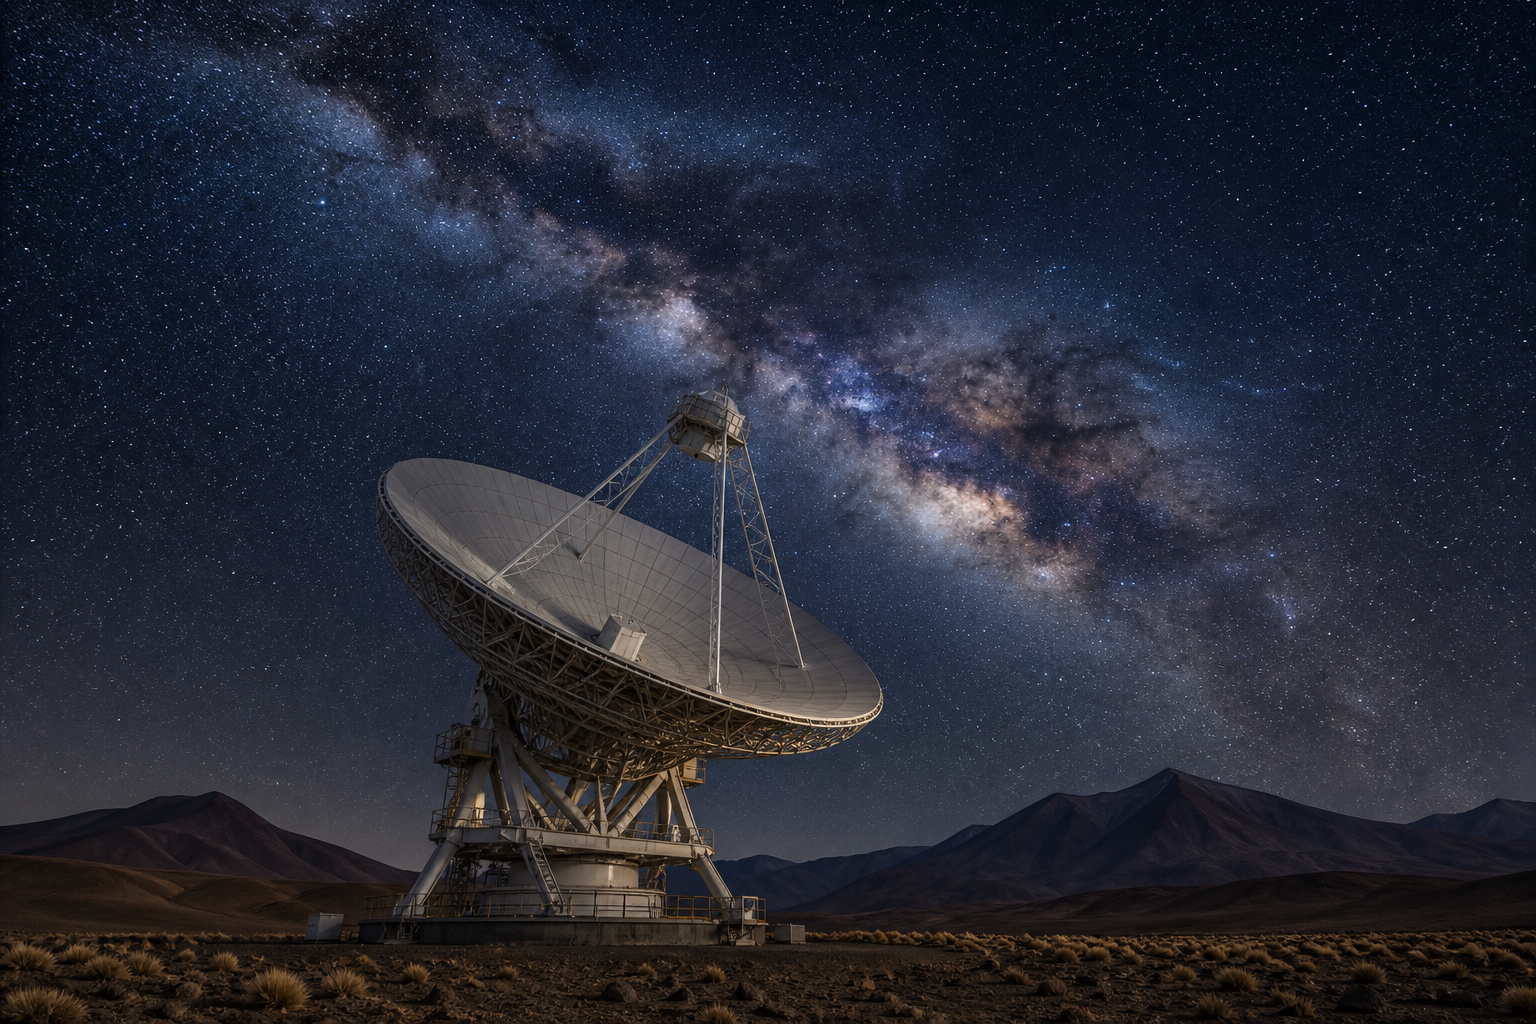
\includegraphics[width=0.58\linewidth]{images/book5/ai/b5-10-radio-dish.png}

{\small A millimetre-wave dish under the Milky Way: the galaxy it listens to, hanging above it. Radio astronomy found the \omterm{def:b3:astrophysics:hubble}{cosmic microwave background} --- the \qty{2.7}{K} hiss that turned out to be the beginning.}
\end{omfigure}

\begin{omfigure}
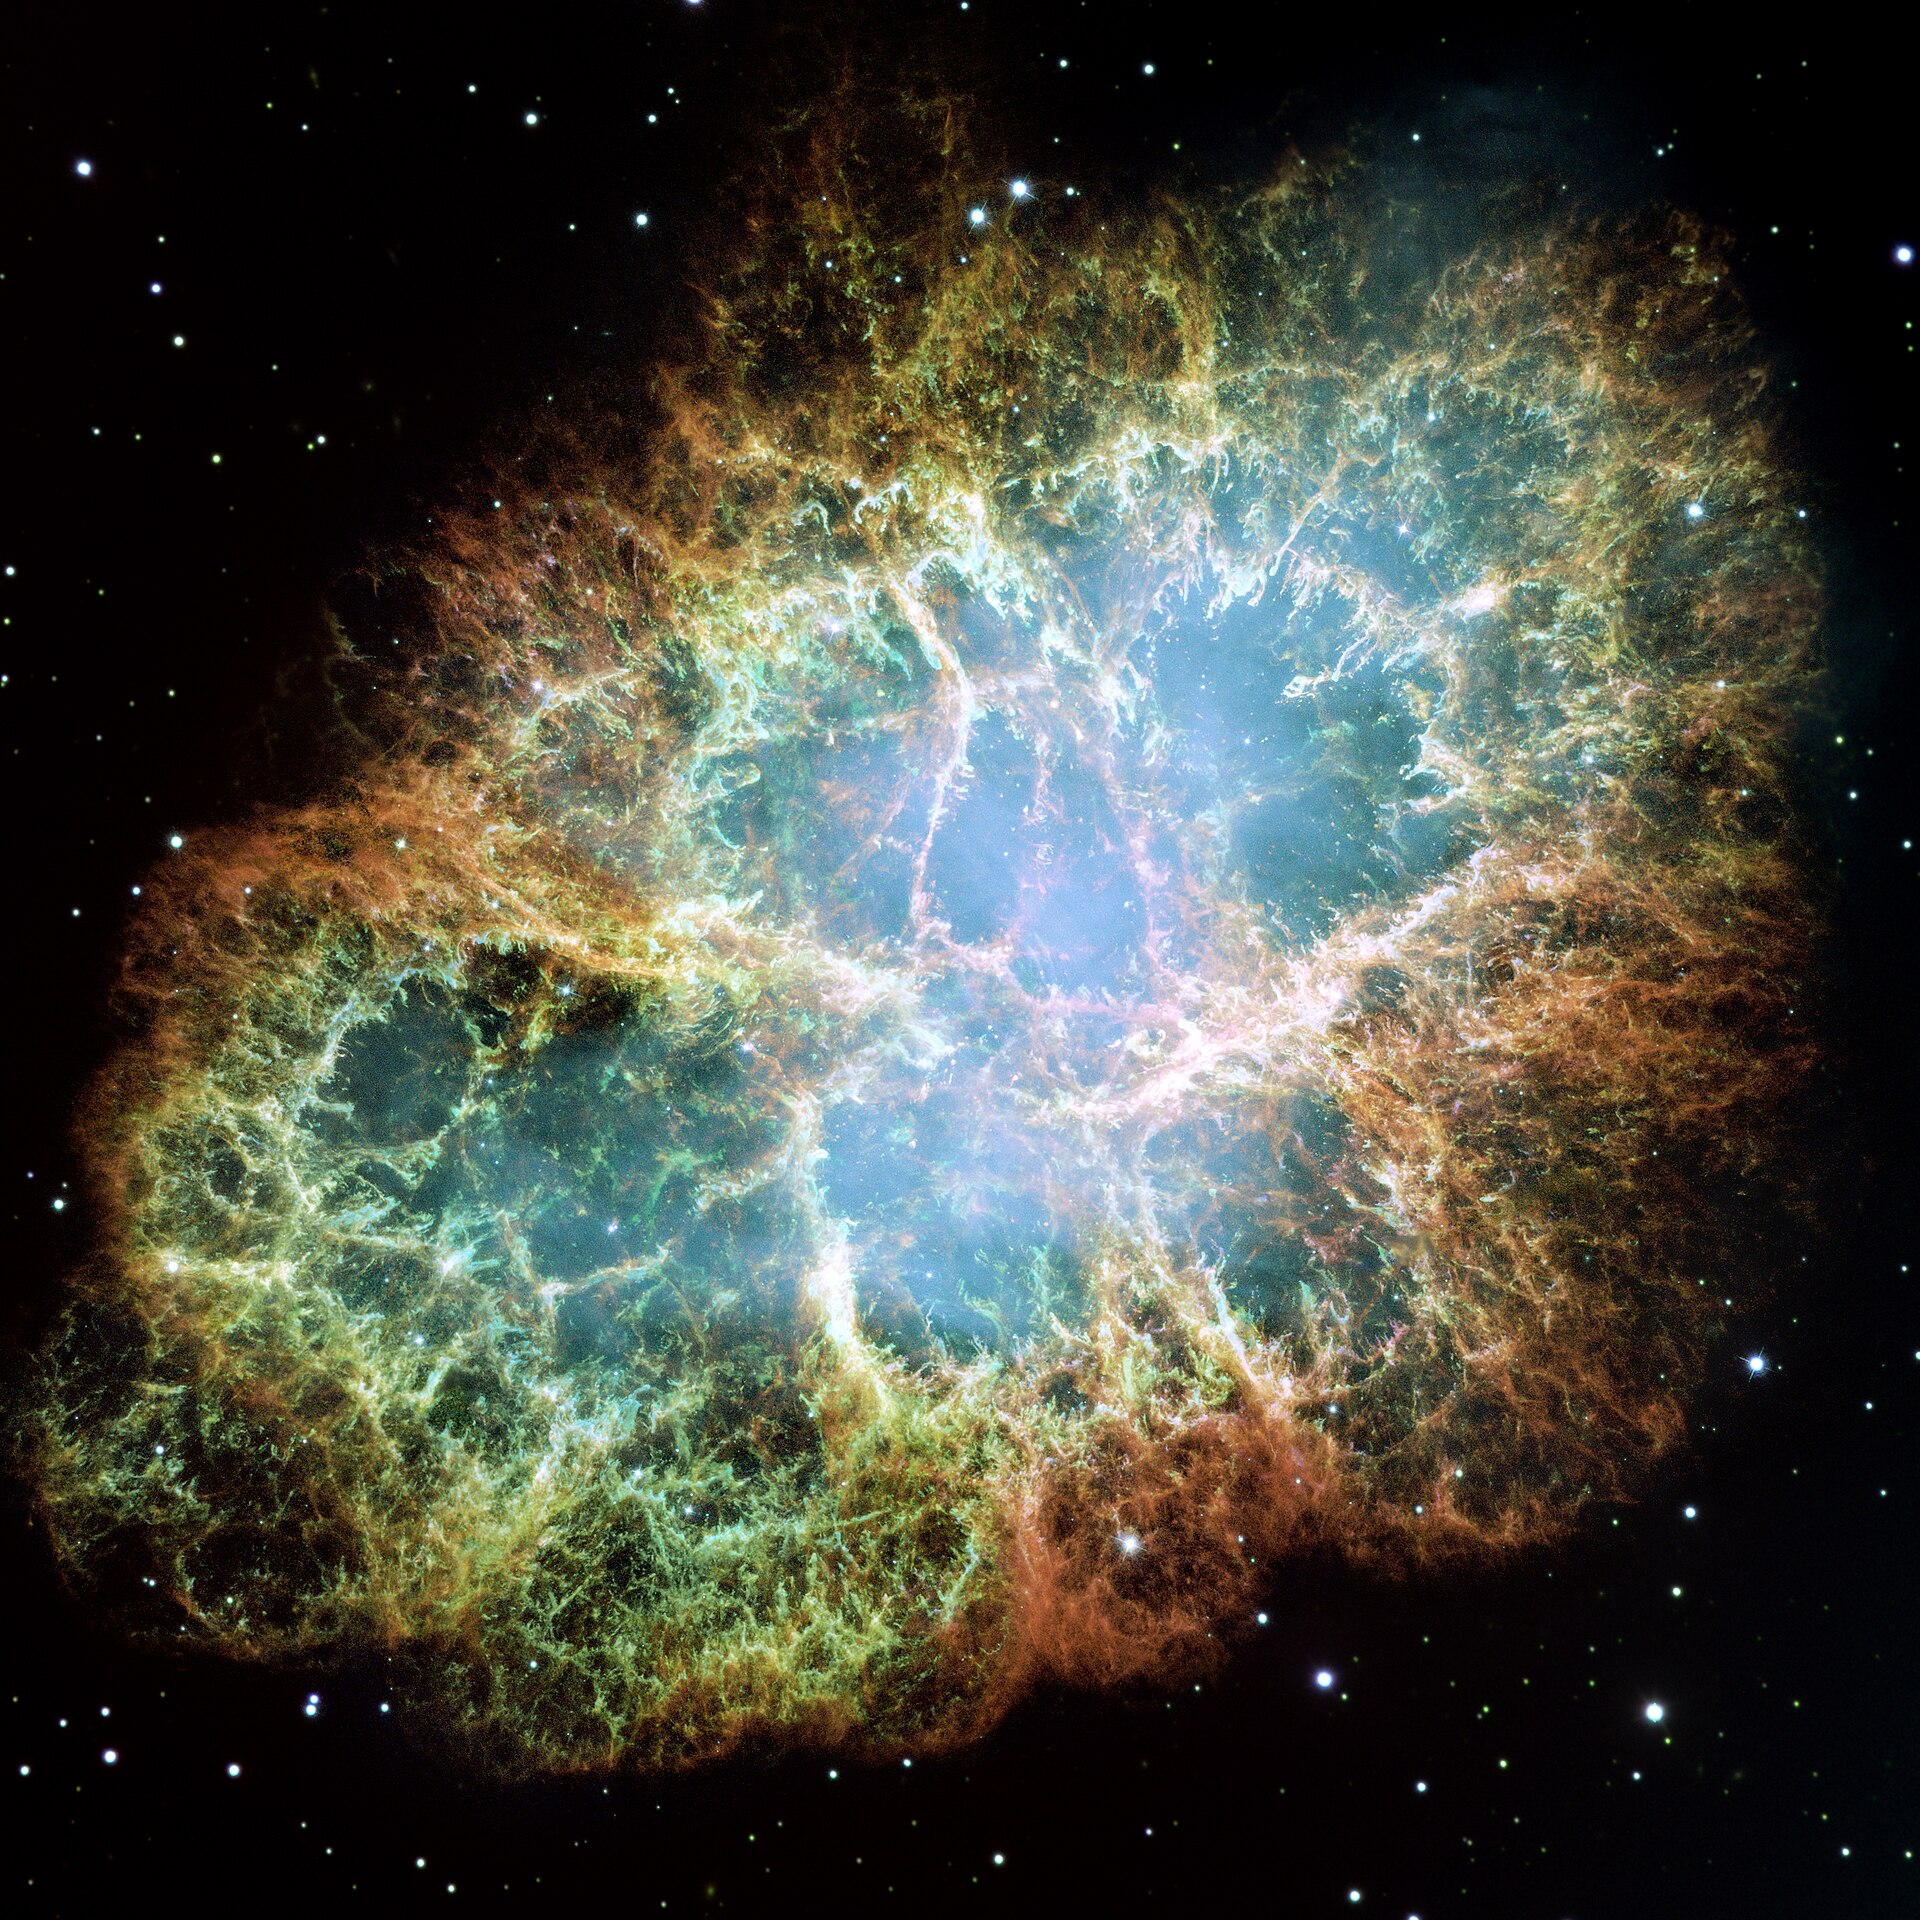
\includegraphics[width=0.6\linewidth]{images/book5/photo-crab-nebula.jpg}

{\small The Crab Nebula (NASA, ESA, J. Hester and A. Loll, public domain): the wreckage of the 1054 supernova, still expanding, with the millisecond lighthouse of a \omterm{prop:b3:astrophysics:compact}{neutron star} at its heart --- the weekend problem, photographed nine centuries later.}
\end{omfigure}

\section{Problem: The night the star died}

\begin{problem}\label{pb:b3:astrophysics:1}
\emph{The night the star died.} On 23 February 1987, a blue
supergiant in the Large Magellanic Cloud --- $d \approx
\qty{50}{kpc} \approx \qty{1.5e21}{m}$ --- became SN~1987A, the
nearest supernova in four centuries. Hours \emph{before} any
telescope saw it brighten, three underground detectors counted
two dozen neutrinos. You are reconstructing that night from first
principles.

\medskip\noindent\textbf{Part I --- The star that was.}

\begin{enumerate}
  \item The progenitor weighed ${\sim}20\,M_\odot$. Using
        \cref{exo:b3:astrophysics:4}'s scaling, estimate its
        lifetime and compare with the Sun's.
  \item By its last day the star was an onion: H, He, C, O, Si
        shells around an iron core. Why does each successive
        fuel require a hotter core?
  \item Why does the sequence stop, permanently, at iron?
        (\cref{prop:b3:nuclear-physics:binding}.)
  \item The inert iron core grows toward $1.4\,M_\odot$. What is
        special about that number, and what pressure fails
        there?
  \item Silicon burning sustains the star for about a
        \emph{day}: what does that say about how a star's
        clock accelerates toward the end?
  \item Once pressure support fails, roughly how long does free
        fall take, for a core of density
        $\sim\qty{e12}{kg/m^3}$ ($t \sim 1/\sqrt{G\rho}$)?
\end{enumerate}

\medskip\noindent\textbf{Part II --- The neutrino flash.}

\begin{enumerate}[resume]
  \item The core ($M \approx 1.4\,M_\odot = \qty{2.8e30}{kg}$)
        collapses to $R \approx \qty{12}{km}$: compute the
        gravitational energy released, $E \sim GM^2/R$.
  \item Compare with the light of a billion suns shining for a
        month ($L \sim 10^{9}L_\odot$ for $\qty{2.6e6}{s}$):
        show the photons are a rounding error --- where do the
        99\,\% go, and why can only neutrinos escape a
        collapsing core promptly?
  \item Spread $E \approx \qty{3e46}{J}$ over a sphere of
        radius \qty{1.5e21}{m}: compute the energy fluence at
        Earth.
  \item With $\sim\qty{15}{MeV}$ per neutrino, compute the
        number fluence (neutrinos per \unit{m^2}).
  \item A detector holds \qty{2000}{t} of water:
        ${\sim}1.5\times10^{32}$ free protons. With an
        interaction probability per proton of
        $\sigma \approx \qty{1e-46}{m^2}$ per antineutrino
        (given), estimate the expected count --- and compare
        with the eleven that one detector logged.
  \item The neutrinos beat the light by hours. Explain both
        clocks: what delays the photons (where is the
        brightening actually born?), and what does the
        \omterm{def:b3:relativistic-kinematics:event}{near-simultaneity} say about the neutrino's mass and
        speed?
  \item Twenty-five counted neutrinos: state, in one sentence
        each, two things they confirmed about supernova theory.
\end{enumerate}

\medskip\noindent\textbf{Part III --- What is left.}

\begin{enumerate}[resume]
  \item Compute the mean density of the \qty{12}{km},
        $1.4\,M_\odot$ remnant and compare with
        \cref{def:b3:nuclear-physics:nuclide}'s nuclear
        density.
  \item The progenitor core spun once per 30 days at
        $R \sim \qty{e5}{km}$: estimate the remnant's period.
  \item Its magnetic field, flux-frozen, is amplified by
        $(R_0/R)^2$: from \qty{e-2}{T}, compute the surface
        field.
  \item Explain the lighthouse: what sweeps, what beams, and
        why the Crab pulsar (born 1054, chronicled as a daytime
        ``guest star'') still flashes thirty times a second.
  \item Had the remnant exceeded ${\sim}3\,M_\odot$: compute
        $R_{\text{s}}$ for $3\,M_\odot$ and state its fate.
  \item Pulsar timing is stable to $10^{-15}$: name one physics
        use of a clock that good, spinning in the sky.
\end{enumerate}

\medskip\noindent\textbf{Part IV --- What it means.}

\begin{enumerate}[resume]
  \item The oxygen you breathe and the iron in your blood:
        trace each atom's biography in two sentences, from
        big-bang hydrogen to your bloodstream.
  \item Type Ia supernovae (\omterm{ex:b3:quantum-statistics:dwarf}{white dwarfs} pushed past
        $M_{\text{Ch}}$) all detonate at the same mass, hence
        nearly the same brightness. Explain why that makes them
        \emph{standard candles}, and how
        \cref{def:b3:astrophysics:hubble}'s diagram is built
        from them.
  \item In 1998, distant Ia supernovae came out \emph{dimmer}
        than Hubble's straight line predicts: state the
        conclusion that earned the 2011 Nobel Prize.
  \item Estimate how far SN~1987A's light had travelled when it
        arrived, in years --- and note what was happening on
        Earth when it set out.
  \item The LMC neutrinos passed through you too (everyone
        alive that day). Roughly how many crossed each human
        (${\sim}\qty{0.03}{m^2}$)? Did anyone feel it
        (\cref{exo:b3:particle-physics:10})?
  \item Close the book's ledger in four lines: a star balanced
        for ten million years by tunnelling; a collapse paid
        out in neutrinos; a corpse held up by Pauli; and the
        debris --- including the reader --- still riding
        Hubble's expansion.
\end{enumerate}
\end{problem}
